\documentclass{article}
\usepackage[T1]{fontenc}
\usepackage{lmodern}
\usepackage{graphicx}
\usepackage{amsmath,amssymb}
\usepackage[a4paper,margin=2cm]{geometry}
\usepackage[absolute,overlay]{textpos}
\setlength{\TPHorizModule}{1mm}
\setlength{\TPVertModule}{1mm}
\usepackage[indonesian]{babel}
\usepackage{hyperref}
\setlength{\emergencystretch}{2em}
% unit: Halaman 10

\begin{document}

% === Halaman 10 (llm) ===

Steganografi menyembunyikan eksistensi pesan sehingga keberadaannya tidak diketahui

\vspace{10mm}

\textcolor{red}{\textbf{Keamanan informasi}}

% deskripsi: Foto berbagai macam paprika berwarna hijau, kuning, dan merah yang digunakan sebagai ilustrasi konsep steganografi (menyembunyikan pesan dalam media gambar).
% bbox normalisasi: [0.4650, 0.1930, 0.8970, 0.8060]
\begin{textblock*}{90.72mm}(97.65mm,57.32mm)
\noindent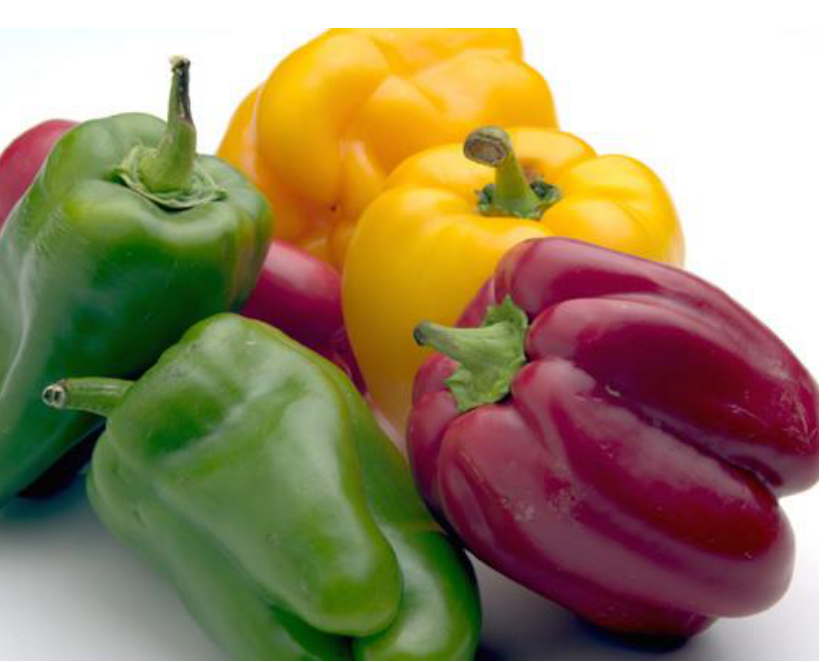
\includegraphics[width=90.72mm,height=182.06mm]{../../images/llm/page_010_img_01.png}%
\end{textblock*}

\end{document}
